\subsection{Bemessungskriterien}
\subsubsection{Anordnung von Leitungsschutzorganen}

Lösen Sie folgende Aufgabenstellungen:
\begin{enumerate}
    \item   \question{An welcher Stelle einer Leitung sind Überstromschutzorgane anzubringen?}\\\\
            Überstromschutzorgane müssen an jeder Stelle, an der einer Veränderung
            \begin{itemize}
                \item des Querschnitts
                \item der Art der Verlegung 
                \item des Leitungsaufbaus
            \end{itemize}
            den zulässigen Dauerstrom $I_Z$ reduziert.

    \item   \question{Darf der N-Leiter mit einem eigenen Überstromschutzorgan abgesichert werden? \\ a) Wird empfohlen \\ b) Ja \\ c) Nein \\[\baselineskip] (Antwort + Begründung + Bedingungen)} \\\\
            Nein. Er darf keine Einzelsicherung beinhalten. Wird der N-Leiter durch eine Auslösung unterbrochen, sind die Geräte zwar nicht funktionsfähig, 
            können aber trotzdem unter Spannung stehen. Bei Fehlersuche: \textbf{Lebensgefahr!}

    \item   \question{Darf der N-Leiter gemeinsam mit dem Überstromschutzorgan der Aussenleiter abgeschaltet werden? \\ a) Wird empfohlen \\ b) Ja \\ c) Nein \\[\baselineskip] (Antwort + Begründung + Bedingungen)} \\\\
            Anhand TAEV 2020/II/53: Wird empfohlen. Die Fehlersuche wird vereinfacht da Stromkreise einfacher lokalisiert werden können. Der Neutralleiter darf zeitlich nicht vor dem Außenleiter ausgeschaltet werden.
            Ähnlich darf der Außenleiter nicht vor dem Neutralleiter eingeschaltet werden.
            
    \item   \question{Darf der PE-Leiter mit einem eigenen Überstromschutzorgan abgesichert werden? \\ a) Wird empfohlen \\ b) Ja \\ c) Nein \\[\baselineskip] (Antwort + Begründung + Bedingungen)} \\\\
            \textbf{\textcolor{red}{Nein!}} Eine Abschaltung des Schutzleiters behindert die Fehlerschutzmaßnahme Fehlerstrom-Schutzschaltung.

    \item   \question{Darf der PE-Leiter gemeinsam mit dem Überstromschutzorgan der Aussenleiter abgesschaltet werden? \\ a) Wird empfohlen \\ b) Ja \\ c) Nein \\[\baselineskip] (Antwort + Begründung + Bedingungen)} \\\\
            \textbf{\textcolor{red}{Nein!}} Eine Abschaltung des Schutzleiters behindert die Fehlerschutzmaßnahme Fehlerstrom-Schutzschaltung.
            Außerdem ist eine Abschaltung des Schutzleiters sinnlos, da dieser im Normalfall sowieso keinen Strom führt.

    \item   \question{\textcolor{red}{Darf der Überstromschutz vom Überlastschutz getrennt werden? (+Beispiel) An welcher Stelle der Leitung können die jeweiligen Schutzorgane angebracht werden?}} \\\\
            Ja, beispielsweise bei Motoren (Thermorelais + Schmelzsicherung). Der Kurzschlusschutz muss immer am Anfang der Leitung angebracht werden. Eine Versetzung ist nur bedingt möglich. Der Überlastschutz
            kann im Zuge der Leitung beliebig verschoben werden.
\end{enumerate}

\subsubsection{Schaltanlage / graphische Symbole}
Lösen Sie die unten aufgelisteten Aufgabenstellungen.

\begin{enumerate}
    \item   \question{Zeichnen Sie das Symbol einer Schmelzsicherung für Drehstromanschluss (einpolige und mehrpolige Darstellung)}
            \begin{figure}[!htp]
                \centering
                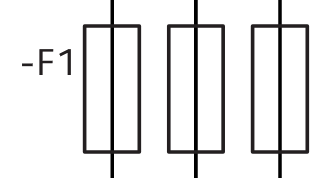
\includegraphics[width = 0.5\textwidth]{img/Schmelzsicherungen.png}
            \end{figure}

            
    \clearpage

    \item   \question{Zeichnen Sie das Symbol eines Leitungsschutzschalters für Drehstromanschluss (einpolige und mehrpolige Darstellung)}
            \begin{figure}[!htp]
                \centering
                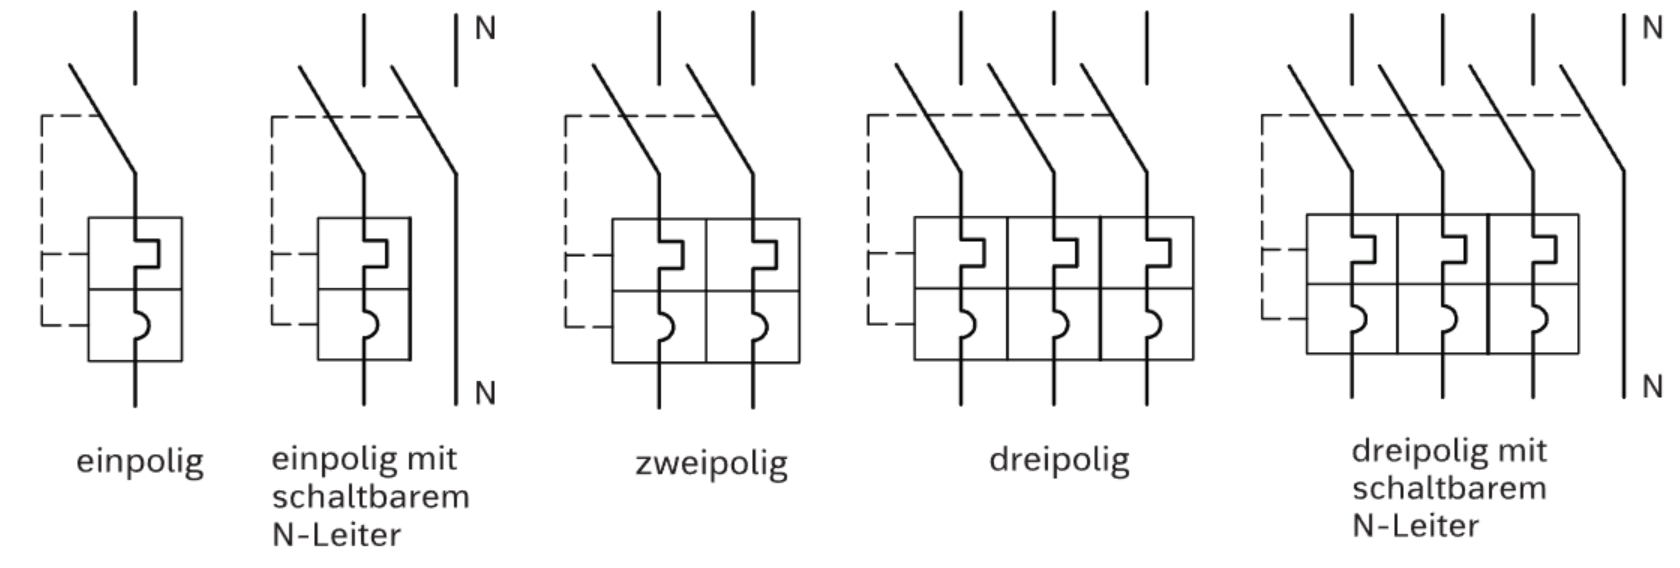
\includegraphics[width = 0.8\textwidth]{img/LSS_symbol.png}
            \end{figure}
            
\end{enumerate}